\documentclass[fr]{../../../eplnotes}

\usepackage{float}
\usepackage{../../../eplmath}
\usepackage{stmaryrd}
\usepackage[french,ruled,vlined]{algorithm2e}

\renewcommand{\S}{\mathcal{S}}
\renewcommand{\contradiction}{\hspace*{\fill}$\lightning$}

\SetKwComment{Comment}{$\triangleright$\ }{}

\hypertitle{Mathématiques discrètes I : Théorie et algorithmique des graphes}{5}{INMA}{1691}
{Gilles Peiffer}
{Raphaël Jungers}[
\paragraph{Remarque} Ce document reprend les notes prises
au cours de l'année 2018-2019.
]

\section{Premier cours magistral}
\subsection{Introduction}
	De façon informelle,
	on peut dire qu'un graphe
	est ``un réseau de sommets reliés par des arêtes''.
	Un exemple d'un graphe serait donc par exemple
	celui à la \figuref{graph}.
	\begin{figure}[H]
	\centering
	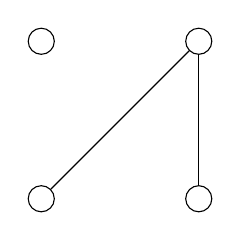
\begin{tikzpicture}
		\node[draw, circle] at (-1,2)  (1) {};
		\node[draw, circle] at ( 1,2)  (2) {};
		\node[draw, circle] at (-1,0)  (3) {};
		\node[draw, circle] at ( 1,0)  (4) {};

		\draw[-] (2) edge node[anchor = north] {} (3);
		\draw[-] (2) edge node[anchor = north east] {} (4);
	\end{tikzpicture}
	\caption{Un graphe à 4 sommets et 2 arêtes.}
	\label{fig:graph}
	\end{figure}

	Pourquoi est-il intéressant d'étudier la théorie des graphes?
	Grâce aux résultats de celle-ci,
	énormément de problèmes semblant initialement compliqués
	sont réduits à des problèmes relativement simples.
	En effet, un acronyme intéressant,
	très souvent valable en théorie des graphes,
	est \textsc{TONCAS}:
	``\emph{The Obviously Necessary Condition is Also Sufficient}'',
	c'est-à-dire que si une condition paraît intuitivement nécessaire,
	il y a de bonnes chances qu'elle soit également suffisante.
\subsection{Définitions}
	\begin{mydef}[Graphe]
		Un \emph{graphe} $G$ est un triplet ordonné $(V, E, \phi)$, où:
		\begin{itemize}
		\item $V$ est un ensemble dont les éléments sont appelés sommets ou noeuds;
		\item $E$ est un ensemble dont les éléments sont appelés arêtes;
		\item $\phi$ est une fonction, dite fonction d'incidence,
		qui associe à chaque arête un sommet ou une \emph{paire} de sommets.
		\end{itemize}
	\end{mydef}
	Prenons de nouveau un exemple de graphe (\figuref{graph_2}).
	\begin{figure}[H]
	\centering
	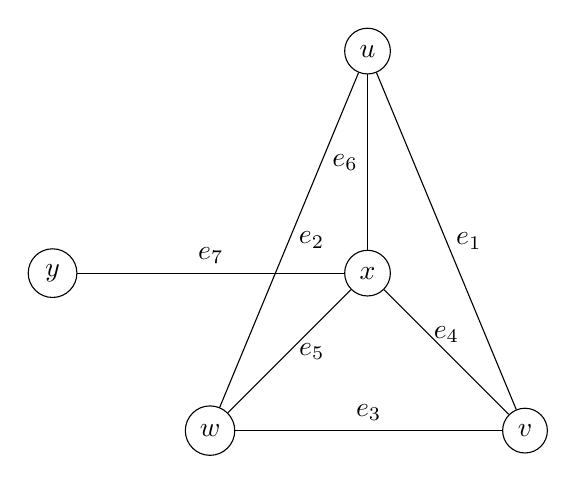
\begin{tikzpicture}
		\node[draw, circle] at ( 0, 2.82)  (u) {$u$};
		\node[draw, circle] at ( 0, 0  )  (x) {$x$};
		\node[draw, circle] at (-4, 0  )  (y) {$y$};
		\node[draw, circle] at ( 2,-2  )  (v) {$v$};
		\node[draw, circle] at (-2,-2  )  (w) {$w$};

		\draw (u) -- (v) node [midway, right] {$e_1$};
		\draw (u) -- (w) node [midway, right] {$e_2$};
		\draw (v) -- (w) node [midway, above] {$e_3$};
		\draw (x) -- (v) node [midway, above] {$e_4$};
		\draw (x) -- (w) node [midway, right] {$e_5$};
		\draw (x) -- (u) node [midway, left] {$e_6$};
		\draw (x) -- (y) node [midway, above] {$e_7$};
	\end{tikzpicture}
	\caption{Un graphe à 5 sommets et 7 arêtes.}
	\label{fig:graph_2}
	\end{figure}

	Pour ce graphe, on a
	\begin{align*}
		V &= \{u, v, w, x, y\}\,,\\
		E &= \{e_1, e_2, \dots, e_7\}\,,\\
		\phi(e_1) &= (u,v)\,,\\
		\phi(e_2) &= (u,w)\,,\\
		&\vdotswithin{=}\\
		\phi(e_7) &= (x,y)\,.\\
	\end{align*}

	\begin{mydef}[Degré]
		Le degré d'un sommet
		est le nombre d'arêtes incidentes à celui-ci.
	\end{mydef}

	\begin{myexem}[Sous-graphe]
		Un exemple de sous-graphe du graphe en \figuref{graph_2}
		est le graphe en \figuref{subgraph}.
		\begin{figure}[H]
		\centering
		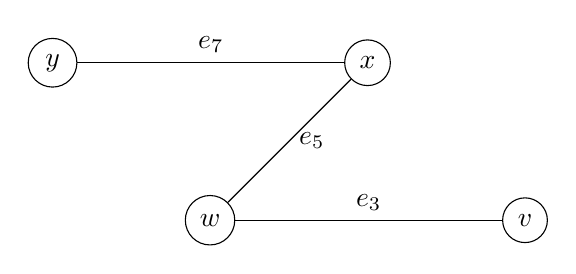
\begin{tikzpicture}
			\node[draw, circle] at ( 0, 0  )  (x) {$x$};
			\node[draw, circle] at (-4, 0  )  (y) {$y$};
			\node[draw, circle] at ( 2,-2  )  (v) {$v$};
			\node[draw, circle] at (-2,-2  )  (w) {$w$};
			\draw (v) -- (w) node [midway, above] {$e_3$};
			\draw (x) -- (w) node [midway, right] {$e_5$};
			\draw (x) -- (y) node [midway, above] {$e_7$};
		\end{tikzpicture}
		\caption{Un graphe chemin à 4 sommets et 3 arêtes,
		sous-graphe de celui à 5 sommets et 7 arêtes en \figuref{graph_2}.}
		\label{fig:subgraph}
		\end{figure}
		En général, un \emph{sous-graphe} du graphe $(V, E, \phi)$
		est un graphe $(V', E', \phi')$ avec :
		\begin{itemize}
		\item $V' \subseteq V$;
		\item $E' \subseteq E$;
		\item $\phi'$ est la restriction de $\phi$ à $E'$.
  \end{itemize}
	\end{myexem}

	\begin{mydef}[Graphe simple]
		Un graphe simple est un graphe sans boucle ni arête multiple.
	\end{mydef}

	Il faut noter qu'un graphe est une notion abstraite,
	indépendante de sa représentation.
	Le graphe $G$ aurait tout aussi bien pu être noté sous la forme
	\begin{figure}[H]
	\centering
	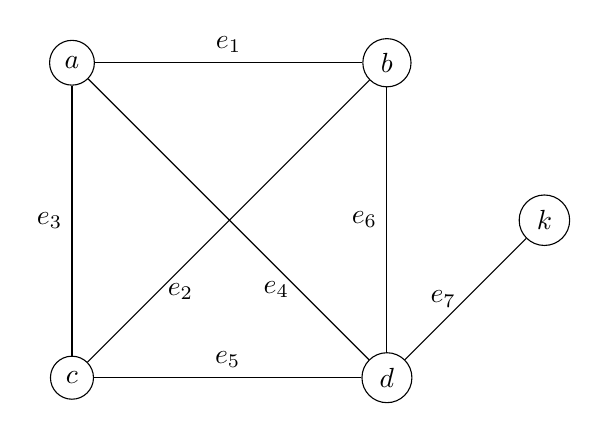
\begin{tikzpicture}
		\node[draw, circle] at ( 2, 2)  (u) {$b$};
		\node[draw, circle] at ( 2,-2)  (x) {$d$};
		\node[draw, circle] at ( 4, 0)  (y) {$k$};
		\node[draw, circle] at (-2, 2)  (v) {$a$};
		\node[draw, circle] at (-2,-2)  (w) {$c$};

		\draw (u) -- (v) node [midway, above] {$e_1$};
		\draw (u) -- (w) node [near end, right] {$e_2$};
		\draw (v) -- (w) node [midway, left] {$e_3$};
		\draw (x) -- (v) node [near start, left] {$e_4$};
		\draw (x) -- (w) node [midway, above] {$e_5$};
		\draw (x) -- (u) node [midway, left] {$e_6$};
		\draw (x) -- (y) node [midway, left] {$e_7$};
	\end{tikzpicture}
	\caption{Le graphe de la \figuref{graph_2} représenté différemment.}
	\label{fig:graph_2_iso}
	\end{figure}

	L'\emph{isomorphisme} est
	\[
	\begin{array}{cc}
		y & k \\
		x & d \\
		w & c \\
		u & b \\
		v & a
	\end{array}
	\]

	\subsection{Isomorphisme de graphes}
	\begin{mydef}[Isomorphisme de graphes]
		Deux graphes $(V, E, \phi)$ et $(V', E', \phi')$
		sont dits \emph{isomorphes} s'il existe
		des bijections $f \colon V \to V'$ et $g \colon E \to E'$ telles que:
		\[
		\phi(e) = (u,v) \iff \phi(g(e)) = \big(f(u),f(v)\big)\,.
		\]
		Deux graphes sont isomorphes
		s'il y a une bijection entre les n\oe{}uds et les arêtes.
	\end{mydef}

	\begin{mypropo}[La relation d'isomorphisme est une relation d'équivalence]
		Toute relation d'équivalence satisfait à 3 conditions:
		\begin{itemize}
			\item elle est réflexive;
			\item elle est symétrique;
			\item elle est transitive.
		\end{itemize}
		Prouvons que la relation d'isomorphisme de graphes
		est une relation d'équivalence.
		\begin{proof}
			Commençons par prouver la réflexivité.
			Cela revient à dire qu'il y a un isomorphisme
			entre le graphe et lui-même.
			Pour prouver cela,
			il suffit de remarquer
			qu'un isomorphisme satisfaisant cette propriété
			est la permutation identité,
			car elle satisfait $G_1 \simeq G_2$.
			\bigbreak
			Prouvons maintenant la symétrie de l'isomorphisme.
			Soit $f \colon V(G_1) \to V(G_2)$,
			alors $f^{-1}$ est un isomorphisme de $G_2 \to G_1$.
			En effet, on sait que
			\[
			uv \in E(G_1) \iff f(u)f(v) \in E(G_2)\,.
			\]
			On sait alors que $\forall x,y \in V(G_2)$
			\[
			f^{-1}(x)f^{-1}(y) \in E(G_1) \iff xy \in E(G_2)\,.
			\]
			\bigbreak
			Finalement, prouvons la transitivité.
			Supposons que $f \colon V(F) \to V(G)$
			et $g \colon V(G) \to V(H)$.
			On a alors
			\begin{align*}
				uv \in E(F) &\iff f(u)f(v) \in E(G)\\
				\intertext{et}
				f(u)f(v) \in E(G) &\iff g\big(f(u)\big)g\big(f(v)\big) \in E(H)\,.
			\end{align*}
			Cela implique que $g \circ f$
			est une bijection,
			ce qui implique à son tour $F \simeq H$.
			\bigbreak
			En combinant ces trois résultats,
			on remarque donc que l'isomorphisme de graphes
			est une relation d'équivalence.
		\end{proof}
	\end{mypropo}

	\begin{mypropo}[$G \simeq H \iff \widebar{G} \simeq \widebar{H}$]
		La preuve est immédiate en observant
		que toute non-arête de $G$ sera également
		une non-arête de $H$.
		Ce petit truc permet parfois
		de voir relativement facilement
		si deux graphes sont isomorphes,
		bien qu'en général,
		cela reste une tâche compliquée.
		% TODO add graphs
	\end{mypropo}
	\subsection{Théorème d'Euler}
	Un des nombreux théorèmes dus à Leonhard Euler
	est l'observation qu'un graphe connexe est eulérien
	si et seulement si le degré de tous ses sommets est pair.
	\begin{mytheo}[Théorème d'Euler]
		Un graphe connexe est eulérien
		si et seulement si le degré de chacun de ses sommets
		est un nombre pair.
		\begin{proof}
		Démontrons l'implication directe d'abord.
		Considérons le problème eulérien
		où en tout n\oe{}ud il y a
		autant d'arêtes entrantes que sortantes.
		(Il s'agit de la condition pour qu'un graphe soit eulérien.)
		Le degré du n\oe{}ud est
		la somme de ce nombre d'arêtes entrantes et sortantes.
		Il sera donc égal à $2n$,
		où $n$ est le nombre d'arêtes entrantes,
		ce qui est toujours un nombre pair.
		\bigbreak
		L'implication indirecte se démontre par construction,
		et se comprend intuitivement par construction.\footnote{C'est vague comme preuve,
		mais il y en a des plus complètes sur Internet,
		notamment dans le syllabus en ligne.}
		\end{proof}
	\end{mytheo}
\section{Deuxième cours magistral}
\subsection{Représentations d'un graphe}
Soit le graphe $G$ de la \figuref{mat}.
\begin{figure}[H]
	\centering
	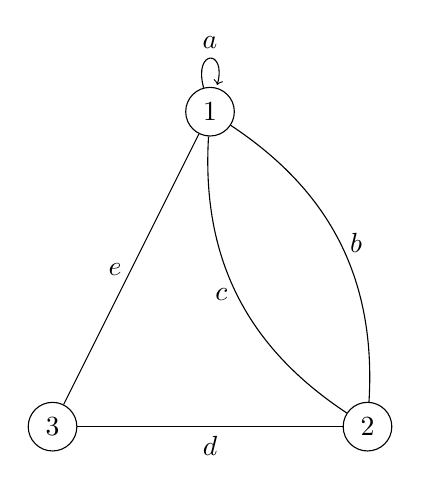
\begin{tikzpicture}
	\node[draw, circle] at ( 0, 4)  (1)  {$1$};
	\node[draw, circle] at ( 2, 0)  (2)  {$2$};
	\node[draw, circle] at (-2, 0)  (3)  {$3$};

	\draw[-] (1) edge [loop above] node {$a$} (1);
	\draw[-] (1) edge [bend left] node [midway,right] {$b$} (2);
	\draw[-] (1) edge [bend right] node [midway,left] {$c$} (2);
	\draw[-] (2) edge node [midway,below] {$d$} (3);
	\draw[-] (1) edge node [midway,left] {$e$} (3);
	\end{tikzpicture}
	\caption{Un graphe.}
	\label{fig:mat}
\end{figure}
On peut représenter ce graphe de deux façons distinctes:
\begin{itemize}
	\item sa \emph{matrice d'incidence} et
	\item sa \emph{matrice d'adjacence}.
\end{itemize}
\begin{mydef}[Matrice d'incidence d'un graphe non orienté]
	La matrice d'incidence d'un graphe non orienté
	est la matrice rectangulaire $M$ de taille $n \times m$
	dont l'élément $m_{ij}$ est
	\begin{itemize}
		\item $1$ si le sommet $v_i$ est une extrémité de l'arête $e_j$;
		\item $2$ si l'arête $x_{j}$ est une boucle sur $v_{i}$;
		\item $0$ sinon.
	\end{itemize}
\end{mydef}
\begin{mydef}[Matrice d'adjacence]
	La matrice d'adjacence d'un graphe $G$ à $n$ sommets
	est la matrice $n \times n$ booléenne $A$
	dont l'élément $a_{ij}$ est
	\begin{itemize}
		\item $1$ si $v_i v_j \in E$;
		\item $0$ sinon.
	\end{itemize}
\end{mydef}
\bigbreak
Pour le graphe $G$ de la \figuref{mat},
on a donc les représentations suivantes:
\[
A = \bordermatrix{  & 1 & 2 & 3 \cr
                  1 & 1 & 2 & 1 \cr
                  2 & 2 & 0 & 1 \cr
                  3 & 1 & 1 & 0 \cr}\,,
\quad
M = \bordermatrix{  & a & b & c & d & e\cr
                  1 & 2 & 1 & 1 & 0 & 1\cr
                  2 & 0 & 1 & 1 & 1 & 0\cr
                  3 & 0 & 0 & 0 & 1 & 1\cr}\,.
\]

\begin{mytheo}[Théorème des poignées de main]
	La somme des degrés des n\oe{}uds d'un graphe
	est deux fois le nombre d'arêtes.
	Mathématiquement,
	\[
	\sum_{v_i \in V} \deg(v_i) = 2 \abs{E}\,.
	\]
	\begin{proof}
		\begin{align*}
		\sum_{i}\sum_{j} M_{ij} &= \sum_{v_i \in V} \deg(v_i)\\
		&= \sum_j 2\\
		&= 2 \abs{E}\,.\qedhere
		\end{align*}
	\end{proof}
\end{mytheo}

\begin{mytheo}[Matrice d'adjacence et nombre de parcours]
	Soit $A$ la matrice d'adjacence d'un graphe.
	Alors l'élément $a^k_{ij}$ de $A^k$ ($k \ge 0$)
	est le nombre de parcours de longueur $k$
	de $v_i$ vers $v_j$.
	\begin{proof}
		Par induction.
		\begin{description}
			\item[Cas de base.]
			Pour $k = 1$, c'est vrai
			par la définition de la matrice d'adjacence.
			\item[Cas inductif.]
			Supposons la propriété vraie pour $k$.
			Soit
			\begin{itemize}
				\item $i$ et $j$ deux n\oe{}uds,
				\item $\pi^{k+1}_{ij}$ le nombre de parcours
				de $i$ vers $j$ de longueur $k+1$,
				\item  $\epsilon_{ij}$ le nombre d'arêtes
				de $i$ vers $j$ et
				\item $a^k_{ij}$ l'entrée en ligne $i$
				et colonne $j$ de $A^k$.
			\end{itemize}
			On a alors
			\begin{align*}
			\pi^{k+1}_{ij} &= \sum_{l \in V} \pi_{il}^{k} \epsilon_{lj}\\
			&= \sum_{l \in V} a^k_{il} a_{lj}\\
			&= a^{k+1}_{ij}\,.\qedhere
			\end{align*}
		\end{description}
	\end{proof}
\end{mytheo}

\begin{myexem}[Séquences de De Bruijn]
\label{exem:code}
Un autre exemple d'utilisation de la matrice d'adjacence
est qu'elle permet par exemple de répondre à la question
``Combien de mots binaires de longueur $k$ ne contiennent pas `$111$'?''\,.

Prenons le graphe du problème (\figuref{code}),
où chaque n\oe{}ud est la terminaison actuelle du mot,
et où chaque arête indique la terminaison que l'on aurait
en rajoutant soit un $0$ soit un $1$.
\begin{figure}[H]
	\centering
	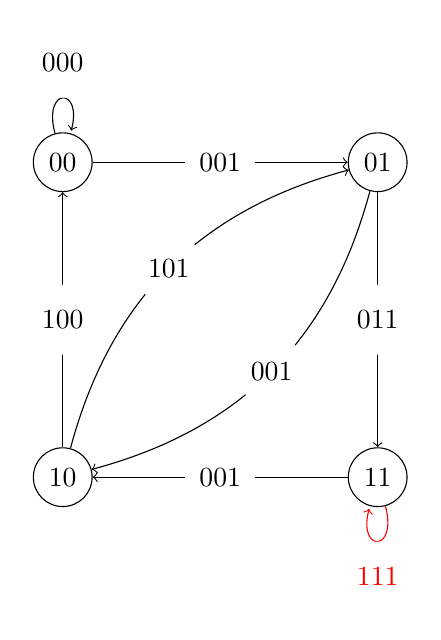
\begin{tikzpicture}
	\node[draw, circle] at (-2, -2)  (10)  {$10$};
	\node[draw, circle] at (-2,  2)  (00)  {$00$};
	\node[draw, circle] at ( 2,  2)  (01)  {$01$};
	\node[draw, circle] at ( 2, -2)  (11)  {$11$};

	\begin{scope}[every node/.style={fill=white,circle}]
		\path[->] (00) edge [loop above] node {$000$} (00);
		\path[->] (11) edge [loop below,red] node {$111$} (11);
		\path[->] (00) edge node {$001$} (01);
		\path[->] (10) edge node {$100$} (00);
		\path[->] (10) edge [bend left] node {$101$} (01);
		\path[->] (01) edge [bend left] node {$001$} (10);
		\path[->] (01) edge node {$011$} (11);
		\path[->] (11) edge node {$001$} (10);
	\end{scope}
	\end{tikzpicture}
	\caption{Graphe de l'Exemple~\ref{exem:code}.
	La seule arête qu'on ne compte pas est celle en rouge,
	car c'est ce cas-là qu'on veut éviter.}
	\label{fig:code}
\end{figure}
On construit la matrice d'adjacence (en ne comptant pas l'arête rouge):
\[
A = \begin{pmatrix}
1 & 1 & 0 & 0\\
0 & 0 & 1 & 1\\
1 & 1 & 0 & 0\\
0 & 0 & 1 & 0
\end{pmatrix}\,.
\]
Maintenant, en calculant les valeurs propres de la matrice $A$,
et en choisissant la plus grande ($\rho \approx 1.84$ en l'occurrence),
on peut trouver la capacité du code.
Pour une longueur $k$,
le nombre de mots ne contenant pas la séquence $111$ est $\approx \rho^k$.
\end{myexem}
\subsection{Graphe biparti}
\begin{mytheo}[Graphe biparti]
\label{theo:bipartite}
	Un graphe est biparti si et seulement si
	tous ses cycles sont de longueur paire.
	\begin{proof}
	\noindent
	\newline
	$\boxed{\implies}$
	\newline
	Soit un graphe $G$ biparti et un cycle $C = v_0, v_1, v_2, \dots, v_0$.
	Supposons $v_0 \in V_0$, $v_1 \in V_1$, $v_2 \in V_0$,\dots.
	Tout cycle termine en $V_0$ et contient donc
	un nombre pair d'arêtes.

	\noindent
	\newline
	$\boxed{\impliedby}$
	\newline
	Soit $v_0$ un n\oe{}ud arbitraire.
	On définit
	\begin{align*}
		V_0 &= \set{v \suchthat d(v,v_0) \textnormal{ est pair}}\\
		V_1 &= \set{v \suchthat d(v,v_0) \textnormal{ est impair}}\,.
	\end{align*}
	Par contradiction.
	Supposons sans perte de généralité $\exists u,v \in V_0$.
	Soient $p,q$ les plus courts chemins
	de $v_0$ à $u$ et $v$ respectivement.
	\begin{figure}[H]
	\centering
	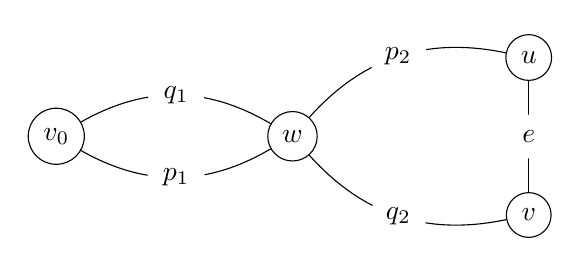
\begin{tikzpicture}
	\begin{scope}[every node/.style={fill=white,circle}]
		\node[draw, circle] at (-4, 0)  (v0)  {$v_0$};
		\node[draw, circle] at (-1, 0)  (w)  {$w$};
		\node[draw, circle] at ( 2, 1)  (u)  {$u$};
		\node[draw, circle] at ( 2,-1)  (v)  {$v$};

		\draw[-] (v0) edge [bend left]  node {$q_1$} (w);
		\draw[-] (v0) edge [bend right] node {$p_1$} (w);
		\draw[-] (w) edge [bend left]  node {$p_2$} (u);
		\draw[-] (w) edge [bend right] node {$q_2$} (v);
		\draw[-] (u) edge node {$e$} (v);
	\end{scope}
	\end{tikzpicture}
	\caption{Le graphe pour la preuve du Théorème~\ref{theo:bipartite}.}
	\label{fig:bipartite}
	\end{figure}
	Soit $w$ le dernier n\oe{}ud dans $p \cap q$.
	Notre \emph{claim} est que $p_2 e q_2$ est un cycle pair.
	Cependant,
	\begin{align*}
	\abs{p_1 p_2 e q_2 q_1} &= \abs{p_1} + \abs{p_2 e q_2} + \abs{q_1}\\
	d(v_0,u) + d(v_0,v) + 1 &= 2 \abs{p_1} + \abs{p_2 e q_2}\,.
	\end{align*}
	Comme le coté de gauche de cette équation est impair
	($u$ et $v$ sont à une distance paire de $v_0$ car ils sont dans $V_0$),
	et que $2 \abs{p_1}$ est évidemment pair,
	le cycle $p_2 e q_2$ doit être impair.
	C'est donc une contradiction,
	ce qui termine la preuve.
	\end{proof}
\end{mytheo}
\begin{mytheo}[Théorème des amis et des étrangers]
	Dans toute fête de six personnes,
	soit au moins trois d'entre eux sont (par paires)
	mutuellement des étrangers,
	soit au moins trois d'entre eux sont (par paires)
	mutuellement des amis\footnote{Ce théorème est un cas particulier
	du théorème de Ramsey, qui a donné lieu
	à une nouvelle branche des mathématiques,
	la théorie de Ramsey.}.

	\begin{proof}
		Si on attribue à chaque personne un sommet dans un graphe,
		et qu'on trace une arête rouge
		si les deux sommets sont ``amis'',
		et une arête bleue si ils sont ``inconnus'',
		on peut raisonner sur ce problème
		comme un problème de théorie des graphes.

		Choisissons un sommet quelconque; appelons-le $P$.
		Il y a cinq arêtes issues de $P$.
		Elles sont de couleur rouge ou bleu.
		Le principe des tiroirs dit
		qu'au moins trois d'entre elles doivent être
		de la même couleur,
		car s'il y a moins de trois d'une couleur,
		disons rouge, alors il y en a au moins trois qui sont bleues.

		Soient $A$, $B$, $C$ les autres extrémités
		de ces trois arêtes,
		toutes de la même couleur, disons bleu.
		Si parmi $AB$, $BC$, $CA$, l'une est bleue,
		alors cette arête,
		avec les deux arêtes joignant $P$
		aux extrémités de cette arête forme un triangle bleu.
		Si aucune parmi $AB$, $BC$, $CA$ n'est bleue,
		alors les trois arêtes sont rouges
		et nous avons un triangle rouge, à savoir, $ABC$.
	\end{proof}
\end{mytheo}

\section{Troisième cours magistral}

\subsection{Plus courts chemins}
\begin{mytheo}[Le plus court parcours entre deux n\oe{}uds
est toujours un chemin]\leavevmode
	\begin{proof}
		Soit $d'$ la longueur du plus court chemin
		et $d$ la longueur du plus court parcours $P$.
		Comme tout chemin est un parcours,
		on a nécessairement $d' \ge d$.

		Supposons, par l'absurde, $d' > d$.
		$P$ n'est donc pas un chemin et contient un ou plusieurs cycles.
		\[
		p = u \ldots \underbrace{v_i \ldots v_i}_{\textnormal{cycle $C$}} \ldots v\,.
		\]
		Si on retire le cycle $C$,
		on obtient le parcours $P' = u \ldots v_i \ldots v$.
		Comme on considère tous les poids positifs,
		on a deux cas possibles:
		\begin{enumerate}
			\item Le cycle $C$ possède au moins une arête
			de poids $w_i > 0$
			$\implies P'$ est plus court que $P$.
			\hspace*{\fill} $\lightning$
			\item Le cycle $C$ est de poids nul
			$\implies P'$ et $P$ ont la même longueur.
			On a donc deux sous-cas:
			\begin{enumerate}[label=(\roman*)]
				\item Il n'y a plus de cycle dans $P'$
				$\implies P'$ est un chemin
				de longueur $d = d'$.
				\hspace*{\fill} $\lightning$
				\item Il reste des cycles dans $P'$.
				On recommence l'argument
				en remplaçant $P$ par $P'$.
				On finira éventuellement sur une contradiction
				car le nombre de cycles dans $P$ est fini.
			\end{enumerate}
		\end{enumerate}
	\end{proof}
\end{mytheo}

\subsection{Algorithme de Dijkstra}
\begin{myexem}
	On cherche les distances à partir de $a$.
	\begin{figure}[H]
	\centering
	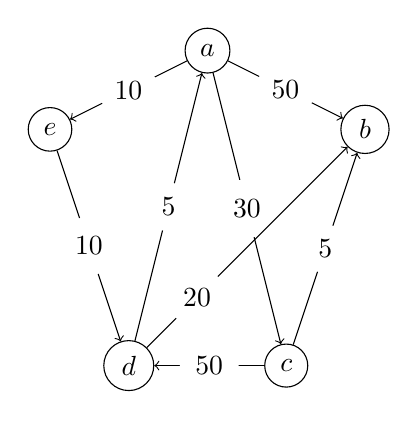
\begin{tikzpicture}
		\node[draw, circle] at (0,  2) (a) {$a$};
		\node[draw, circle] at (2,  1) (b) {$b$};
		\node[draw, circle] at (1, -2) (c) {$c$};
		\node[draw, circle] at (-1,-2) (d) {$d$};
		\node[draw, circle] at (-2, 1) (e) {$e$};
		\begin{scope}[every node/.style={fill=white,circle}]
			\draw[->] (a) edge node {$50$} (b);
			\draw[->] (c) edge node {$5$} (b);
			\draw[->] (c) edge node {$50$} (d);
			\draw[->] (e) edge node {$10$} (d);
			\draw[->] (a) edge node {$10$} (e);
			\draw[->] (d) edge node {$5$} (a);
			\draw[->] (a) edge node {$30$} (c);
			\draw[->] (d) edge node[near start] {$20$} (b);
		\end{scope}
	\end{tikzpicture}
	\caption{Un exemple de digraphe pondéré.}
	\label{fig:dijkstra_graph}
	\end{figure}

	Le graphe de la \figuref{dijkstra_graph} est défini par
	\begin{align*}
	V &= \{a,b,c,d,e\}\,,\\
	E &= \{ab, cb, cd, ed, ae, da, ac\}\,.
	\end{align*}

	\begin{table}[H]
		\centering
		\begin{tabular}{ccccccc}
			\hline
			$u'$ & $S$ & $\ell(a)$ & $\ell(b)$ & $\ell(c)$ & $\ell(d)$ & $\ell(e)$\\
			\hline
			$a$ & $\lbrace a \rbrace$ & $\boxed{0}$ & $\infty$ & $\infty$ & $\infty$ &$\infty$\\
			$e$ & $\lbrace a,e \rbrace$ && 50 & 30 & $\infty$ & $\boxed{10}$\\
			$d$ & $\lbrace a,e,d \rbrace$ && 50 & 30 & $\boxed{20}$ &\\
			$c$ & $\lbrace a,e,d,c \rbrace$ && 40 & $\boxed{30}$ & &\\
			$b$ & $\lbrace a,e,d,c,b \rbrace$ && $\boxed{35}$ & & &\\
			\hline
		\end{tabular}
		\caption{Résultats de l'Algorithme de Dijkstra
		pour le graphe de la \figuref{dijkstra_graph}.}
		\label{tab:dijkstra}
	\end{table}
\end{myexem}

\begin{myrem}
	Les dernières arêtes utilisées pour joindre un sommet
	forment les plus courts chemins.
\end{myrem}

En pseudocode,
l'Algorithme de Dijkstra peut être implémenté comme suit:

\begin{algorithm}[H]
\DontPrintSemicolon
\KwData{$G$, le graphe, et $s$, le n\oe{}ud source.}
\KwResult{Les plus courts chemins de $s$ vers tout autre n\oe{}ud du graphe.}
\Begin{
	crée l'ensemble des n\oe{}uds $\mathcal{Q}$\;
	dist[$s$] $\gets$ 0 \Comment*[r]{Initialisation}

	\ForEach{vertex $v$ in $G$}{
		dist[$v$] $\gets \infty$ \Comment*[r]{Distance inconnue de $s$ à $v$}
		prev[$v$] $\gets$ UNDEFINED \Comment*[r]{Prédécesseur de $v$ sur chemin optimal partant de $s$}
		ajoute $v$ à $\mathcal{Q}$ \Comment*[r]{Tous les n\oe{}uds sont initialement dans $\mathcal{Q}$}
	}
	dist[$s$] $\gets 0$\;
	\While{$\mathcal{Q}$ n'est pas vide}{
		$u \gets$ n\oe{}ud dans $\mathcal{Q}$ avec $\min$ dist[$u$] \Comment*[r]{Enlève et retourne le n\oe{}ud avec la distance minimale dans $\mathcal{Q}$}
		enlève $u$ de $\mathcal{Q}$\;
		\ForEach{voisin $v$ de $u$}{
			alt $\gets$ dist[$u$] $+$ length($u$, $v$)\;
			\If{alt $<$ dist[$v$]}{
				dist[$v$] $\gets$ alt\;
				prev[$v$] $\gets u$\;
			}
		}
	}
	\Return dist[], prev[]\;
}
\caption{Dijkstra($G$, $s$)\label{algo:dijkstra}}
\end{algorithm}

L'Algorithme~\ref{algo:dijkstra} a une complexité de $\bigoh(\abs{V}^2)$.
Il existe aussi des implémentations
avec des structures de données différentes\footnote{Les min-priority queues.},
permettant de réduire la complexité à $\bigoh(\abs{E} + \abs{V} \log \abs{V})$.

\begin{mytheo}[Correction de l'Algorithme de Dijkstra]
	L'Algorithme de Dijkstra est correct et efficace.
	\begin{proof}
	Par induction.
	On suppose les propriétés vérifiées à l'itération $i-1$
	et on veut les prouver pour l'itération $i$.
	Soit $\S_i$ l'ensemble $\S$ à l'itération $i$.
	\noindent
	\newline
	\fbox{Cas de base ($i = 1$)}
	\newline
	À la fin de l'initialisation,
	\begin{align}
	\S &= \{u_0\}\,, \nonumber\\
	\ell(u_0) &= 0 = d(u_0,u_0)\,. \label{eq:dijkstra1}
	\end{align}
	Après la première mise à jour de $\ell$,
	\begin{align}
	\ell(v) &= \min(\ell(v), \underbrace{\ell(v_0)}_{=0} {} + w(u_0 v))\,, \quad \forall v \in \S \nonumber\\
	\implies \ell(v) &= \infty \textnormal{ si il n'y a pas d'arête } v_0v. \label{eq:dijkstra2}
	\end{align}
	\noindent
	\newline
	\fbox{Cas inductif}
	\newline
	$u_i$ est le n\oe{}ud qui vient d'être rajouté à l'itération précédente.
	Il faut prouver qu'après avoir rajouté $u_i$ dans $\S_i$,
	$\ell(u_i) = d(u_0, u_i)$.

	La condition~\eqref{eq:dijkstra1} est verifiée
	par les autres éléments de $\S_i$
	par l'hypothèse d'induction.
	Supposons par l'absurde que l'algorithme
	n'a pas trouvé le plus court chemin vers $u_i$
	et que donc $\ell(u_i) > d(u_0, u_i)$.

	Par la condition~\eqref{eq:dijkstra2} appliquée à l'itération $i-1$,
	$\ell(u_i)$ est la longueur du plus court chemin
	où tous les n\oe{}uds internes sont dans $\S_{i-1}$.

	Si $\ell(u_i) \ne d(u_0, u_i)$,
	alors il y a un autre plus court chemin
	qui passe par un n\oe{}ud de $\widebar{S_{i-1}}$.
	Soit $v$ le premier n\oe{}ud de $\widebar{S_{i-1}}$ de ce chemin.
	% Using mathcal makes the widebar command broken for some reason...
	Comme $u \ldots v \ldots u_i$ est un plus court chemin,
	$u_0 \ldots v$ en est aussi un.
	On sait que $\ell(v) = d(u_0, v)$
	car tous les n\oe{}uds internes de $u_0 \ldots v$
	sont uniquement dans $\S_{i-1}$
	(par \eqref{eq:dijkstra2} à l'étape $i-1$).
	De plus, on sait que les poids sont $\ge 0$.
	\[
	\implies \ell(v) = d(u_0, v) \le d(u_0, u_i)\,.
	\]

	Mais $u_i$ est tel que
	\[
	\ell(u_i) = \min\limits_{u \in \widebar{S_{i-1}}}(\ell(u))\,.
	\]
	On a donc $\ell(u_i) \le \ell(v) \le d(u_0, u_i)$.
	\contradiction

	Commençons par montrer que
	\[
	\ell(v) \ge d(u_0, v)\,, \quad \forall v \in \S\,.
	\]
	Les seuls $\ell(v)$ qui changent à cette itération
	sont égaux à
	\[
	\ell(v) = \underbrace{\ell(u_i)}_{= d(u_0, u_i)} {} + w(u_i v)\,,
	\]
	qui ont la longueur du chemin $u_0 \ldots u_i v$.
	Donc, $\ell(v) \ge d(u_0, v)$.
	Montrons que $\ell(v)$ est la longueur du plus court chemin
	dont tous les n\oe{}uds internes sont dans $\S$.

	Par \eqref{eq:dijkstra2} à l'étape $i-1$,
	$\ell(v)\,, \quad \forall v \notin \S_{i-1}$
	est longueur du plus court chemin de $u_0$ à $v$
	dont tous les n\oe{}uds internes appartiennent à $\S_{i-1}$.

	Il faut juste considérer les chemins passant par $u_i$.
	Le plus court de ces chemins est le chemin fait
	du plus court chemin de $u_0$ à $u_i$ et de l'arête $u_i v$,
	de longueur $d(u_0, u_i) + w(u_i v)$.
	Le plus court chemin vers $v$ dont les n\oe{}uds internes
	sont dans $\S_i$ a donc soit
	ses n\oe{}uds internes uniquement dans $\S_{i-1}$ (longueur $\ell(v)$),
	soit il passe par $u_i$ (longueur $\ell(u_i) + w(u_i v)$).
	Cela correspond à la mise à jour de $\ell(v)$.
	\[
	\ell(v) = \min(\ell(v), \ell(u_i) + w(u_i v))\,.\qedhere
	\]
	\end{proof}
\end{mytheo}

\begin{mypropo}[Complexité de l'Algorithme de Dijkstra] \leavevmode
	L'Algorithme de Dijkstra est en $\bigoh(\abs{V}^2)$
	\begin{proof}\leavevmode
		\begin{itemize}
			\item Après l'initialisation,
			$\abs{\widebar{\S}} = \abs{V}-1$
			et à chaque passage de boucle décroit de $1$
			$\implies \abs{V}-1$ itérations.
			\item À chaque itération,
			l'opération ``$\forall v \notin \S$'' est
			$\bigoh(\abs{V} - \abs{\S})$, tout comme
			l'opération ``trouver $v_{\textnormal{min}}$''.
			\item Le nombre total d'opérations est donc
			$2 (\abs{V} - 1) + 2 (\abs{V} - 2) + \cdots + 2
			\in \bigoh(\abs{V}^2)$.
		\end{itemize}
		L'algorithme est polynomial
		et donc \emph{relativement} efficace.
	\end{proof}
\end{mypropo}

\subsection{Anneaux et semi-anneaux}

\begin{mydef}[Semi-anneau]
  Un \emph{semi-anneau} est un ensemble
  muni de deux opérations ($\oplus,\otimes$)
  et ses propriétés.
\end{mydef}

\begin{mydef}[Anneau]
  Un \emph{anneau} est un ensemble
  muni de trois opérations ($\oplus,\otimes,\ominus$)
  et ses propriétés.
\end{mydef}

\begin{mydef}[Corps]
  Un \emph{corps} est un ensemble
  muni de quatre opérations ($\oplus,\otimes,\ominus,\oslash$)
  et ses propriétés.
\end{mydef}

\begin{myform}[Autre formule pour le plus court chemin]
	En prenant $A$ tel que $a_{ij} = w(i j)$
	et $w(i j) = \infty$ si il n'y a pas d'arête $ij$.

	On a
	\begin{align*}
		A \oplus B &= \Big(a_{ik} \oplus b_{kj}\Big)_{ij}\,,\\
		A \otimes B &= \Big(\sum_k a_{ik} \otimes b_{kj}\Big)_{ij}\,.
	\end{align*}
	Le $\oplus$ définit la somme matricielle
	et le $\otimes$ définit le produit matriciel.
	Prenons $\oplus = \min$ et $\otimes = +$.
	Le neutre du minimum est $+\infty$
	et le neutre de l'addition est $0$.
	Définissons donc
	\[
	I =
	\begin{pmatrix}
	0 & +\infty & \cdots & +\infty\\
	+\infty & \ddots & \ddots & \vdots\\
	\vdots & \ddots & \ddots & +\infty\\
	+\infty & \cdots & +\infty & 0
	\end{pmatrix}\,.
	\]

	On définit alors
	\begin{align*}
		A \otimes A &= \Big(\min\limits_{k}\big(a_{ik} + a_{kj}\big)\Big)_{ij}\\
		&= \min\limits_{k}\big(w(i k) + w(k j)\big)\\
		&= \textnormal{plus court chemin de deux arêtes.}
	\end{align*}
	et en général, la matrice des plus courts chemins est donnée par
	\[
	I \oplus A \oplus \cdots \oplus A^{\otimes n}\,.
	\]
	Pour calculer le plus court chemin,
	on peut définir alors l'itération:
	\begin{align*}
	M_0 &= I\,,\\
	M_1 &= I \oplus (M_0 \otimes A)\,,\\
	M_2 &= I \oplus (M_1 \otimes A)\,,\\
	&\vdotswithin{=}\\
	M_{k+1} &= I \oplus (M_k \otimes A)\,.
	\end{align*}
	On a fini de converger quand $M_k = M_{k+1}$.
	L'Algorithme de Dijkstra peut être vu
	comme une manière efficace d'implémenter cette itération.
\end{myform}

\section{Quatrième cours magistral}
\subsection{Arbre sous-tendant}
\begin{mydef}[Arbre]
	Un \emph{arbre} est un graphe connexe sans cycle.
	Une \emph{forêt} est un graphe sans cycle.
\end{mydef}
\begin{mydef}[Sous-graphe sous-tendant]
	Un \emph{sous-graphe sous-tendant} d'un graphe $G$
	est un sous-graphe qui contient tous les sommets de $G$.
\end{mydef}

\begin{mytheo}[Tout graphe connexe contient un arbre sous-tendant]\leavevmode
	\label{theo:spanning_tree}
	\begin{proof}
	Soit $G$ un graphe connexe.
	Parmi tous les sous-graphes sous-tendants connexes de $G$,
	on choisit un sous-graphe $G'$,
	minimal pour l'inclusion dans cet ensemble.
	Pour que $G'$ soit un arbre,
	il faut qu'il soit connexe et acyclique.
	\begin{itemize}
		\item Il est connexe par construction.
		\item Supposons que $G'$ ait un cycle.
		Soit $e = uv$ une arête du cycle.
		Si on enlève $e$,
		le graphe est toujours connexe.
		Pour tout parcours $x \ldots uv \ldots y$,
		on peut remplacer $e$ par le reste du cycle.
		\contradiction
	\end{itemize}
	\end{proof}
\end{mytheo}

\begin{mylem}[Feuilles d'un arbre]
	\label{lem:leaves}
	Tout arbre avec au moins deux sommets
	a aux moins deux feuilles (n\oe{}uds de degré un)
	et supprimer une feuille d'un arbre à $n$
	n\oe{}uds produit un arbre à $n-1$ n\oe{}uds.
	\begin{proof}
		Dans un graphe acyclique avec au moins deux sommets,
		les extrémités d'un chemin maximal n'ont pas d'autres voisins
		que leurs voisins sur le chemin.
		Ces extrémités sont donc des feuilles.

		Soit $v$ une feuille d'un arbre $G = (V, E, \phi)$.
		Soit $G' = (V', E', \phi') = G - v$.
		Comme un sommet de degré un
		n'appartient à aucun chemin reliant deux autres sommets,
		pour tout $u,v \in V'$,
		tout chemin de $u$ à $v$ dans $G$ est aussi dans $G'$.
		$G'$ est donc connexe.

		Puisque supprimer un sommet ne peut pas créer de cycle,
		$G'$ est également acyclique.
	\end{proof}
\end{mylem}

\subsection{Caractérisations des arbres}
\begin{mytheo}[Caractérisations des arbres]
	Soit $G$ un graphe à $n$ sommets et $m$ arêtes.
	Alors les conditions suivantes sont équivalentes.
	\begin{enumerate}[label=(\arabic*)]
		\item \label{conn_acy} $G$ est connexe et sans cycle.
		\item \label{acy_mn1} $G$ est sans cycle et $m = n - 1$.
		\item \label{conn_mn1} $G$ est connexe et $m = n-1$.
		\item \label{conn_del}$G$ est connexe
		et supprimer une arête quelconque déconnecte $G$.
		\item \label{acy_add} $G$ est sans cycle
		et ajouter une arête quelconque crée un et un seul cycle.
		\item \label{link} Deux n\oe{}uds de $G$ sont toujours reliés
		par un seul chemin.
	\end{enumerate}
	La dernière condition implique que $G$ est sans boucle
	(pour deux n\oe{}uds identiques).

	\begin{proof}
		\noindent
		\newline
		\newline
		\fbox{\ref{conn_acy} $\implies$ \ref{acy_mn1}}
		\newline
		Par récurrence sur $n$.
		Pour $n = 1$, $m = 0$.
		On a donc bien $m = n - 1$.

		On suppose \ref{acy_mn1} vrai pour $n-1$.
		Pour tout arbre de $n$ n\oe{}uds,
		on trouve une feuille $x$.
		On enlève $x$ et son arête
		et on obtient par le Lemme~\ref{lem:leaves}
		un arbre de $n-1$ n\oe{}uds
		et $n-2$ arêtes (par la récurrence).
		Tout arbre de $n$ n\oe{}uds a donc $n-1$ arêtes.

		\noindent
		\newline
		\fbox{\ref{acy_mn1} $\implies$ \ref{conn_mn1}}
		\newline
		Soient $G_1 = (V_1, E_1, \phi_1),
		\ldots, G_k = (V_k, E_k, \phi_k)$
		les $k$ composantes connexes de $G = (V, E, \phi)$
		avec $n_i = \abs{V_i}$ et $m_i = \abs{E_i}$
		pour $i = 1, \ldots, k$.

		On a
		\[
		\sum_{i=1}^{k} n_i = n
		\quad \textnormal{et} \quad
		\sum_{i=1}^{k} m_i = m\,.
		\]
		Chaque composante satisfait \ref{conn_acy},
		et donc $m_i = n_i - 1$ pour $i = 1, \ldots, k$.
		\begin{align*}
			\implies m &= \sum_{i=1}^{k} m_i \\
			&= \sum_{i=1}^{k} \big(n_i - 1\big) \\
			&= n - k\,.
		\end{align*}
		Or $m = n - 1$,
		ce qui implique $k = 1$.
		Le graphe est donc connexe.

		\noindent
		\newline
		\fbox{\ref{conn_mn1} $\implies$ \ref{conn_del}}
		\newline
		Supposons qu'en enlevant une arête $e$ à $G$,
		le graphe $G' = G - e$ reste connexe.
		Par le Théorème~\ref{theo:spanning_tree},
		$G'$ a un arbre sous-tendant $A$.
		Par \ref{conn_acy} $\implies$ \ref{acy_mn1},
		$A$ a $n - 1$ arêtes.
		$G'$ a au moins $n - 1$ arêtes et $G$ a au moins $n$ arêtes.
		Or, $G$ a $n - 1$ arêtes,
		ce qui implique que $G - e$ n'est pas connexe.
		\contradiction

		\noindent
		\newline
		\fbox{\ref{conn_del} $\implies$ \ref{acy_add}}
		\newline
		Supposons qu'il y ait un cycle dans $G$.
		On peut alors supprimer une arête de ce cycle,
		en gardant la propriété de convexité,
		ce qui contredit l'hypothèse.
		$G$ est donc acyclique.
		\contradiction

		Ajouter une arête quelconque crée un et un seul cycle.
		\begin{itemize}
			\item On montre qu'ajouter une arête $e$
			entre $u$ et $v$ crée un cycle.
			Par connexité,
			il existe un chemin $C$ entre $u$ et $v$ dans $G$.
			On a $u \ldots v e u$ qui est un cycle.
			\item C'est le seul cycle.
			Supposons qu'on ait obtenu au moins deux cycles
			$C_1$ et $C_2$ en ajoutant $e$.
			Si c'est le cas,
			on peut adjoindre $C_1 - e$ et $\widebar{C_2 - e}$
			pour former un parcours fermé $u \ldots v \ldots u$.
			\contradiction
		\end{itemize}

		\noindent
		\newline
		\fbox{\ref{acy_add} $\implies$ \ref{link}}
		\newline
		Supposons qu'il existe deux chemins
		$P_1 = u \ldots v$ et $P_2 = u \ldots v$,
		alors $u \ldots v \ldots u$ est un parcours fermé
		dont on peut extraire un cycle.
		Il y a donc au plus un chemin entre $u$ et $v$.
		\contradiction

		Prouvons maintenant l'existence de ce chemin.
		Si on ajoute une arête entre $u$ et $v$,
		alors par hypothèse on crée un cycle $C$.
		Cela implique que $C - e$ est un chemin entre $u$ et $v$.

		\noindent
		\newline
		\fbox{\ref{link} $\implies$ \ref{conn_acy}}
		\newline
		$G$ est d'office connexe.
		Il suffit donc de montrer qu'il est également acyclique.
		Supposons qu'il existe un cycle.
		Soient $x$ et $y$ deux n\oe{}uds de ce cycle.
		Le cycle donne deux chemins différents de $x$ à $y$.
		$G$ est donc sans cycle.
		\contradiction
		
	\end{proof}
\end{mytheo}

\subsection{Énumération des arbres sous-tendants}
\begin{myform}[Formule de Cayley]
	Soit $T(G)$ le nombre d’arbres sous-tendants de $G$
	et $e$ une arête quelconque de $G$
	qui n’est pas une boucle.
	Alors
	\[
	T(G) = T(G - e) + T(G \cdot e)\,.
	\]
	$G - e$ désigne le graphe avec l'arête $e$ enlevée.
	$G \cdot e$ désigne le graphe
	avec les n\oe{}uds reliés par $e$ fusionnés.
	\begin{proof}
		On divise les arbres sous-tendants de $G$ en deux catégories:
		\begin{enumerate}[label=(\alph*)]
			\item \label{subtract} ceux qui ne contiennent pas $e$;
			\item \label{contract} ceux qui contiennent $e$.
		\end{enumerate}
		On compte les arbres de chaque catégorie.
		\begin{itemize}
			\item Les arbres de \ref{subtract} sont en bijection
			avec les arbres sous-tendants de $G - e$.
			\item Les arbres de \ref{contract} sont en bijection
			avec les arbres sous-tendants de $G \cdot e$.
		\end{itemize}
		On a donc
		\[
		T(G) = T(G - e) + T(G \cdot e)\,.\qedhere
		\]
	\end{proof}
\end{myform}

\begin{mytheo}[Arbres sous-tendants de $K_n$]
	Le \emph{graphe complet à $n$ n\oe{}uds}, noté $K_n$,
	a $n^{n-2}$ arbres sous-tendants.
	C'est également un théorème de Cayley.
\end{mytheo}

\subsection{Arbre sous-tendant de poids minimum}
On a un algorithme naïf tournant en $\bigoh(n^{n-2})$ pour $n$ n\oe{}uds,
mais on peut faire beaucoup mieux.

\subsubsection{Algorithme de Kruskal}
\begin{algorithm}[H]
\DontPrintSemicolon
\KwData{$G$, une graphe pondéré à $n$ n\oe{}uds avec poids $\ge 0$.}
\KwResult{Le graphe formé des arêtes $T$
est un arbre sous-tendant de poids minimum.}
\Begin{
	sort($E$)\Comment*[r]{On trie les arêtes par poids croissant}
	$T \gets \emptyset$\;

	\While{$\abs{T} < n - 1$}{
		$e \gets$ l'arête pas encore considérée de moindre poids\;
		\If{$T \cup \{e\}$ acyclique}{
			$T \gets T \cup \{e\}$\;
		}
	}
	\Return $T$\;
}
\caption{Kruskal($G$)\label{algo:kruskal}}
\end{algorithm}

\begin{mytheo}[Correction de Kruskal]
	L'Algorithme de Kruskal est correct et efficace.
	\begin{proof}
		Soit $T = \{e_1, e_2, \ldots, e_m\}$
		l'ensemble des arêtes de l'arbre trouvé par Kruskal,
		avec les arêtes dans cet ordre.
		C'est bien un arbre sous-tendant
		car il a $n - 1$ arêtes et pas de cycle.

		On suppose que $T$ n'est pas optimal
		et que $T^*$ soit un arbre optimal.
		Soit $e_i$ la première arête choisie pour $T$
		mais absente dans $T^*$.

		$T^*$ est un arbre optimal
		qui contient $e_1, e_2, \ldots, e_{i-1}$ mais pas $e_i$.
		Il y a donc un seul cycle dans $T^* + e_i$.
		Il y a forcément une arête de ce cycle qui n'est pas dans $T$,
		sinon $T$ aurait un cycle.
		On l'appelle $e'$.

		Montrons que le sous-graphe
		avec les arêtes $e_1, e_2, \ldots, e_{i-1}, e'$
		n'a pas de cycle puisqu'il est inclus dans $T^*$.
		Au moment de choisir $e_i$,
		l'algorithme n'a pas choisi $e'$,
		qui pourtant ne crée pas de cycle (donc $w(e') \ge w(e_i)$).

		On considère donc l'arbre $T^* + e_i - e'$.
		C'est un arbre sous-tendant puisqu'il a $n - 1$ arêtes
		et pas de cycles.
		$T^* + e_i - e'$ est au moins aussi léger que $T^*$
		et contient $\{e_1, e_2, \ldots, e_{i-1}, e_i\}$.
		\contradiction

	\end{proof}
\end{mytheo}
C'est un algorithme glouton (\emph{greedy}),
c'est-à-dire qu'à chaque itération,
il vise l'optimum local.
\begin{mypropo}[Complexité de l'Algorithme de Kruskal]
	L'Algorithme de Kruskal requiert un temps de calcul
	de l'ordre de $\bigoh(m \log m)$ sur un graphe à $m$ arêtes.
	C'est le tri qui prend le plus de temps.
	Une implémentation efficiace de la détection de cycles utilise
	une structure de données appelée \emph{ensembles disjoints}.
\end{mypropo}

\subsubsection{Algorithme de Prim}
\begin{algorithm}[H]
\DontPrintSemicolon
\KwData{$G$, une graphe pondéré à $n$ n\oe{}uds avec poids $\ge 0$.}
\KwResult{Le graphe formé des arêtes $T$
est un arbre sous-tendant de poids minimum.}
\Begin{
	$T \gets v$\Comment*[r]{$v$ est un n\oe{}ud de départ arbitraire}

	\While{$\abs{T} < n - 1$}{
		$e \gets$ l'arête de moindre poids incidente à exactement un n\oe{}ud de $T$\;
		$T \gets T \cup \{e\}$\;
	}
	\Return $T$\;
}
\caption{Prim($G$)\label{algo:prim}}
\end{algorithm}

\begin{mytheo}[Correction de Prim]
	L'Algorithme de Prim est correct et efficace.
	% TODO proof
\end{mytheo}

\begin{mypropo}[Complexité de l'Algorithme de Prim]
	L'Algorithme de Prim requiert un temps de calcul
	de l'ordre de $\bigoh(m + n \log n)$
	sur un graphe à $n$ n\oe{}uds et $m$ arêtes.
	Une implémentation efficiace de la sélection d'arêtes utilise
	une structure de données appelée \emph{file de priorité}
	implémentée par un ``tas de Fibonacci''.
\end{mypropo}
\end{document}
